\chapter{Design and Implementation}
The implementation of each part of the system was made with application of Test Driven Development which guarantees full test coverage for the code. Used testing framework is \textit{mocha} \url{https://mochajs.org/}. For creation of doublers (mocks, stubs and spies) for object and method was used \textit{sinon.js }\url{http://sinonjs.org/}. 
Robet Cecil Martin\cite{MartinASD} defined symptoms of not agile design:
\begin{itemize}
	\item Rigidity - The design is difficult to change;
	\item Fragility - The design is easy to break;
	\item Immobility - The design is difficult to reuse;
	\item Viscosity - It is difficult to do the right thing;
	\item Needless complexity - Overdesign;
	\item Needless repetition - Mouse abuse;
	\item Opacity - Disorganized expression;
\end{itemize}
To avoid creation of such software John Dooley \cite{Dooley} and Rober Cecil Maritn \cite{MartinASD} defined  the principles of agile architecture.
\begin{itemize}
	\item Closing - Encapsulate things in your design that are likely to change.
	\item Code to an Interface - rather then to an implementation. 
	\item Do not repeat yourself - Avoid duplicate code.
	\item The Single-Responsibility Principle - A class should have only one reason to change from the business perspective;
	\item The Open/Closed Principle - Software entities (classes, modules, functions, etc.) should be open for extension but closed for modification
	\item The Liskov Substitution Principle - Subtypes must be substitutable for their base types.
	\item The Dependency-Inversion Principle - 		
	\begin{itemize}
		\item High-level modules should not depend on low-level modules.  Both should depend on abstractions. 
		\item Abstractions should not depend upon details. Details should depend upon abstractions.
	\end{itemize}
	\item The Interface Segregation Principle - Clients should not be forced to depend on methods they do not use.
	\item Principles of Least Knowledge - Talk to your immediate friends. 
	\item Principle of Loose Coupling - object that interact should be loosely coupled with well-defined intefaces.
\end{itemize}

This principles have a suggestional nature and can not be strictly followed due to their mutually exclusive nature. Correspondence to each of them will be provided in the end of each section within this chapter.

For description of data structures processed by the system we will use following module (Listing: \ref{demo}) which implements stack with asynchronous methods (respond time for each method is 10 milliseconds). Usage of \textit{setTimeout()} method guaranties its asynchronism while the fact that timeframe for response hardcoded into scraping scripts guarantees that this method is valid for usage as a proof of concept in current research topic.
\lstinputlisting[
language=Javascript, numbers=left, stepnumber=5, firstnumber=1, breaklines=true, 
basicstyle=\footnotesize,
numberstyle=\tiny,
caption={stack.js},
captionpos=b,
label=demo
]
{code/demo/stack.js.txt}
The Test Sheet for test coverage of this module looks as following (Figure: \ref{fig:demoTS}). Note that this test coverage was made with purpose to show handling of asynchronous testing of real-time software but not to cover stack module. There are both types of comparison in invocation line \textbf{D}. Red arrows indicates references withing this test sheet.
\begin{figure}[H]
\centering
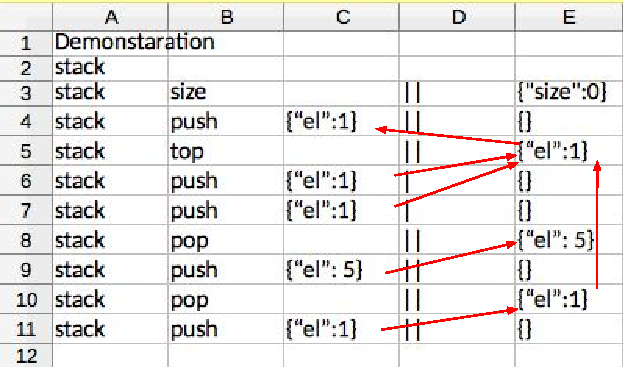
\includegraphics[width=\linewidth]{grafiken/demoTS.pdf}
\caption{Test Sheet coverage for stack.js}
\label{fig:demoTS}
\end{figure}



\section{Read Stream}

This part of the system is an implementation of combining streams pattern. From the internal view it consists of two streams. First stream performs recursive search for files in a provided directory and returns array with absolute paths to them. Second stream reads content of files with \textit{xlsx} module \url{https://www.npmjs.com/package/xlsx} and meta data of the file using embedded node.js module \textit{fs} and pushes it to the up stream.

%\lstinputlisting[
%language=Javascript, numbers=left, stepnumber=5, firstnumber=1, breaklines=true, 
%basicstyle=\footnotesize,
%numberstyle=\tiny,
%caption={read\_stream.js},
%captionpos=b,
%label=demo
%]
%{code/lib/stream/readStream.js.txt}
The \textbf{function getFilesStream} creates readable stream for reading content of directory including nested directories and returns it. 
The \textbf{variable getDataStream} defined by stream in a object mode. For every file path it accepts from the down stream  checks its extensions if its .xlsx then it reads it and obtains first sheet from the book, and reads meta data of the file and pushes it to the up stream.
This two streams are piped in to combined stream using module \textit{multipipe} \url{https://www.npmjs.com/package/multipipe} and returned by the function exported by this module.
In other words, this module exports function which accepts path to the directory and returns array of deferred values each of which is a javascript object with following structure (Listing \ref{readOut})
\lstinputlisting[
language=Javascript, numbers=left, stepnumber=5, firstnumber=1, breaklines=true, 
basicstyle=\footnotesize,
numberstyle=\tiny,
caption={Read Stream Output  / Transform Stream Input JSON},
captionpos=b,
label=readOut
]
{code/readOut.js.txt}

\subsection{Test Coverage}
Following test cases can show each step incrementally performed during the develop process. All calls to systems I/O (e. g. read file meta data, read file) are implemented using stubs. \textbf{Stub} is an implementation of \textit{proxy pattern} which allows to redefine functions behavior. This gives an opportunity to improve speed of tests by replacing functions with call to I/O with empty functions.
%\lstinputlisting[
%language=Javascript, numbers=left, stepnumber=5, firstnumber=1, breaklines=true, 
%basicstyle=\footnotesize,
%numberstyle=\tiny,
%caption={Test coverage for read\_stream.js},
%captionpos=b,
%label=readTest
%]
%{code/test/readStream.js.txt}

The result of tests execution  for this module is following (Fig.: \ref{fig:testRead}):
\begin{figure}[H]
	\centering
	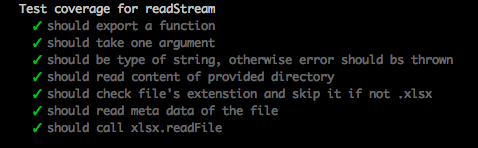
\includegraphics[width=\linewidth]{grafiken/testReadStream.png}
	\caption{Test coverage for read\_stream.js}
	\label{fig:testRead}
\end{figure}



\subsection{Correspondence to design principles}
\begin{itemize}
	\item Closing - module exports single function which returns stream.
	\item Code to an Interface - calls are done to the public functions of required objects. 
	\item Do not repeat yourself - no code duplication;
	\item The Single-Responsibility Principle - can be changed only due to the change of input type (e. g. another spreadsheet type)
	\item The Open/Closed Principle - new pipes can be added in a single place;
	\item The Liskov Substitution Principle - no inheritance;
	\item The Dependency-Inversion Principle - 
		\begin{itemize}
			\item Higher level module \textit{index.js} does not depend on implementation current library
			\item Current library depends on the input type provided by the \textit{index.js}
		\end{itemize}
	\item The Interface Segregation Principle - no calls of unnecessary methods;
	\item Principles of Least Knowledge - communication done only with xlsx files;
	\item Principle of Loose Coupling - communication is done via standard file system and standard stream interfaces.
\end{itemize}
%\begin{itemize}
%	\item Closing - stream is closed over file extension, schema\_maker - object structure returned by 	\textit{xlsx} library;
%	\item Code to Interface - stream obtains and returns values via standard stream interface, call to file system made via standard nodeJS File System stream interface;
%	\item Do not Repeat Yourself - no code duplication;
%	\item Single Responsibility Principle - can be changed only due to the change of input type;
%	\item Open Close Principle - new pipes can be added in a single place;
%	\item Liscov Substitution Principle - no inherited objects used;
%	\item Interface Segregation Principle - no dependency on redundant methods;
%	\item Dependency Inversion Principle - higher level module index.js does not depend on current library
%	\item Least Knowledge Principle - communication to interfaces and invocation of used library;
%	\item Loose Coupling Principle - standard interfaces;
%\end{itemize}
%
%\textbf{Design principles implication:}
%\begin{itemize}
%\item  S. - Single Responsibility Principle - can be changed only due to the change of input type
%\item  O. - Open Close Principle - new pipes can be added in a single place
%\item  L. - Liscov Substitution Principle - no inheritance
%\item  I. - Interface Segregation Principle - Stream interface / File System interface
%\item  D. - Dependency Inversion Principle - Higgher level module index.js does not depend on current library
%
%Writer structure:\\


\section{Transform Stream}
This part of the system performs translation of the Test Sheet in to executable javascript code. In this realization of the Test Sheet concept translation performed in a four stages. 


\lstinputlisting[
language=Javascript, numbers=left, stepnumber=5, firstnumber=1, breaklines=true, 
basicstyle=\footnotesize,
numberstyle=\tiny,
caption={Transform Stream},
captionpos=b,
label=writeIn
]
{code/lib/stream/transformStream.js.txt}

The first stage necessary for the translation is a creation of \textit{schema} object of the Test Sheet. Next stage is detection of execution order. The third step is merging results from previous steps. The last stage is an application of a template to the content of Test Sheet together with the file name of the xlsx file and execution schema created on a previous stage. The result of this transformation is pulled by the downstream as a \textit{content} property of an object together with \textit{meta data} and \textit{fileName} obtained from the upstream (Listing: \ref{writeIn}).

\lstinputlisting[
language=Javascript, numbers=left, stepnumber=5, firstnumber=1, breaklines=true, 
basicstyle=\footnotesize,
numberstyle=\tiny,
caption={Transform Stream Output / Write Stream Input JSON},
captionpos=b,
label=writeIn
]
{code/writeIn.js.txt}

\subsection{Test Coverage}
Following test cases can show each step incrementally performed during the develop process. All calls to systems I/O (e. g. read file meta data, read file) are implemented using stubs. \textbf{Stub} is an implementation of \textit{proxy pattern} which allows to redefine functions behavior. This gives an opportunity to improve speed of tests by replacing functions with call to I/O with empty functions.
%\lstinputlisting[
%language=Javascript, numbers=left, stepnumber=5, firstnumber=1, breaklines=true, 
%basicstyle=\footnotesize,
%numberstyle=\tiny,
%caption={Test coverage for transform\_stream.js },
%captionpos=b,
%label=writeIn
%]
%{code/lib/stream/transformStream.js.txt}

The result of test execution:
\begin{figure}[H]
	\centering
	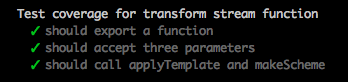
\includegraphics[width=\linewidth]{grafiken/testTransform.png}
	\caption{Test coverage for transform\_stream.js}
	\label{fig:testTransofm}
\end{figure}

\subsection{Correspondence to design principles}
\begin{itemize}
	\item Closing - module exports stream object only;
	\item Code to an Interface - function invocation done via public functions of imported methods. 
	\item Do not repeat yourself - no code duplication;
	\item The Single-Responsibility Principle - can be changed only due to the change of Test Sheet type;
	\item The Open/Closed Principle - new pipes can be added in a single place with adding new functions to be wrapped in them;
	\item The Liskov Substitution Principle - no inheritance;
	\item The Dependency-Inversion Principle - 
				\begin{itemize}
					\item Higher level module \textit{index.js} does not depend on implementation current library;
					\item Current library depends on the input type provided by the \textit{index.js};
				\end{itemize}
	\item The Interface Segregation Principle -  no calls of unnecessary methods;
	\item Principles of Least Knowledge - direct communication done only with helper functions for schema creation and content generation. 
	\item Principle of Loose Coupling - communication is done via the standard stream interface
\end{itemize}


\section{Schema}
This part of the system creates a schema object from the Test Sheet object, the only parameter accepted by the main function of this module is a Test Sheet object (the content of xlsx file). Due to the structure of object was taken decision to perform creation of the schema in two stages.

The \textbf{first stage} is creation of javascript object with Test Sheet properties (e. g. \textit{description, moduleUnderTest, objectsUnderTest, methodsUnderTest, inputs, outputs, invocations}) value of each property except \textit{description} and \textit{moduleUnderTest} are arrays of string with values which represent cell addresses for representative property of the Test Sheet. For the first two properties the values are strings with values (in a Test Sheet) from the cells \textit{A1} and \textit{A2} respectively(Listing: \ref{firstScheme}).

\lstinputlisting[
language=Javascript, numbers=left, stepnumber=5, firstnumber=1, breaklines=true, 
basicstyle=\footnotesize,
numberstyle=\tiny,
caption={Result of the first stage of Test Sheet scheme creation},
captionpos=b,
label=firstScheme
]
{code/firstSchema.js.txt}

The \textbf{sectod stage} is a pivot transformation of the scheme provided by the result of previous stage. The output of this transformation is an object with properties as a numbers of rows in the Test Sheet object. The values for first and second properties are values of \textit{description} and \textit{module} under test from the respective Test Sheet. While all next are objects which consists of following Test Sheet properties: \textit{objectUnderTest, methodUnderTest, inputs, outputs, invocations}. With values as single element arrays with coordinate of respective cell (Listing \ref{scheme}).
\lstinputlisting[
language=Javascript, numbers=left, stepnumber=5, firstnumber=1, breaklines=true, 
basicstyle=\footnotesize,
numberstyle=\tiny,
caption={Result of the scheme creation  for Test Sheet},
captionpos=b,
label=scheme
]
{code/scheme.js.txt}

%\lstinputlisting[
%language=Javascript, numbers=left, stepnumber=5, firstnumber=1, breaklines=true, 
%basicstyle=\footnotesize,
%numberstyle=\tiny,
%caption={Module for creation of the Test Sheet scheme},
%captionpos=b,
%label=writeIn
%]
%{code/lib/scheme/index.js.txt}
\subsection{Test Coverage}
Following test cases can show each step incrementally performed during the develop process. All calls to systems I/O (e. g. read file meta data, read file) are implemented using stubs. \textbf{Stub} is an implementation of \textit{proxy pattern} which allows to redefine functions behavior. This gives an opportunity to improve speed of tests by replacing functions with call to I/O with empty functions.
%\lstinputlisting[
%language=Javascript, numbers=left, stepnumber=5, firstnumber=1, breaklines=true, 
%basicstyle=\footnotesize,
%numberstyle=\tiny,
%caption={Test coverage for creation of the Test Sheet scheme},
%captionpos=b,
%label=writeIn
%]
%{code/test/scheme.js.txt}

The result of test execution:
\begin{figure}[H]
	\centering
	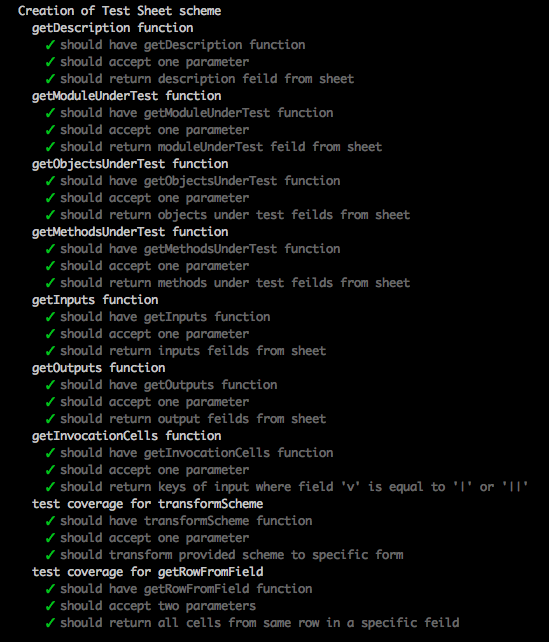
\includegraphics[width=\linewidth]{grafiken/testScheme.png}
	\caption{Test coverage for scheme.js}
	\label{fig:testScheme}
\end{figure}

\subsection{Correspondence to design principles}
\begin{itemize}
	\item Closing - comparison type is closed within the \textit{getInvocationCells} function.
	\item Code to an Interface - exports single function. 
	\item Do not repeat yourself - no code repetition .
	\item The Single-Responsibility Principle - no reason to be changed
	\item The Open/Closed Principle - violated due to the two types comparison;
	\item The Liskov Substitution Principle - no inheritance.
	\item The Dependency-Inversion Principle - does not have any lower level modules;
	\item The Interface Segregation Principle - does not have any lower level modules;
	\item Principles of Least Knowledge - can be invoked only via direct import;
	\item Principle of Loose Coupling - exports single function;
\end{itemize}

\section{Execution Order}
This part of the system is responsible for definition of test steps execution. In general case the execution order of tests within a Basic Test Sheet is defined by the order of test steps. 
Further all Test Sheets support references which provides an ability to define input for one test step as an output of some of the previous steps.


However, in \textit{asynchronous} software the moment when execution is completed comes after the period of time when next function is invoked. Moreover, \textit{real-time} systems have time constraints on their execution together with non-deterministic behavior. This two facts forces to define moment of each test step execution depending on the source of their input parameters. 


For definition of test steps execution order was taken decision to separate test steps in two types. \textit{The first} type covers test steps whose behavior does not make influence to next steps (do not define input parameters for further test steps) and is not determined by any of previous test steps. \textit{The second} type covers test steps which execution result determines behavior of next test steps or defined by previous steps.

%
% But the fact that in this case Basic Test Sheets are applied  for \textit{asynchronous} testing of \textit{real-time} software together with an ability to 
%This shit is important for application for real time software.
The process of order definition is following. Main function accepts two input parameters: \textit{sheet} - the content of xlsx file which defines test sheet and \textit{scheme} - the object generated by the main function from \textit{scheme.js} file (Listing: \ref{order}). Walking through the scheme elements stating with the third (skipping service rows) performs check for each cell in a sheet object for determining is behavior of test step defined by result of any previous test step. In this case such test step will be pushed to the \textit{chain} array as the first element and all dependent test steps will be pushed to the nested array as a list of dependent test steps. If \textit{chain} is not empty it will be pushed to global (in a function scope) \textit{chains}  array. All other rows will be pushed to the \textit{linear array}. Such approach guarantees saving order of rows and creates a record of tree as a list of direct child nodes.


\lstinputlisting[
language=Javascript, numbers=left, stepnumber=5, firstnumber=1, breaklines=true, 
basicstyle=\footnotesize,
numberstyle=\tiny,
caption={Generation of tree structure as a list of childnodes},
captionpos=b,
label=order
]
{code/order.js.txt}

For the further creation of test steps execution order the list of direct child nodes should be merged in to nested list for child nodes which has other child nodes. In terms of test steps this means that result one test step can define behavior of few test steps either directly or via some intermediate test steps. 
The merging process is performed by the \textit{transformation} function (Listing \ref{transformation}). It accepts an array object (\textit{chains} array described previously) and performs iterative walk through with recursive call for each nested array. During each iteration this function iterates through values of childes (nested arrays) and checks is any of them is a parent for other childes (is it present as a first element in next arrays). In such case it takes list of its childes and creates a two dimensional array which replaces the the parent element in a list of childes with removing parent entry together with its childes from the current position. This operation of replacement performed recursively through all nested arrays using \textit{isIn} function which determines is given element a belongs to the provided array including nested arrays.

\lstinputlisting[
language=Javascript, numbers=left, stepnumber=5, firstnumber=1, breaklines=true, 
basicstyle=\footnotesize,
numberstyle=\tiny,
caption={Generation of nested data structure},
captionpos=b,
label=transformation
]
{code/transformFunction.js.txt}

The final step is concatenation of arrays from \textit{first} and \textit{second} test steps types. For our example, rows \textit{one} and \textit{two} belong to the first type as a service rows which does not define any test steps together with rows \textit{three} and \textit{four}. Note that input parameter for the test step defined it a row four is referenced by the expected output of the test step defined in a row five. However, the input parameter can not be changed by the execution process of test step and can be passed to the next step before starting execution without any execution logic violation. In the same time result of test step \textit{five} is an input parameter for the steps \textit{six}, \textit{seven} and \textit{ten} which in turn defines an input for the test step \textit{eleven} (Listing: \ref{orderSteps}).
\lstinputlisting[
language=Javascript, numbers=left, stepnumber=5, firstnumber=1, breaklines=true, 
basicstyle=\footnotesize,
numberstyle=\tiny,
caption={Execution order},
captionpos=b,
label=orderSteps
]
{code/executionOrderSchema.js.txt}


\subsection{Test coverage}

Following test cases can show each step incrementally performed during the develop process.
\begin{figure}[H]
	\centering
	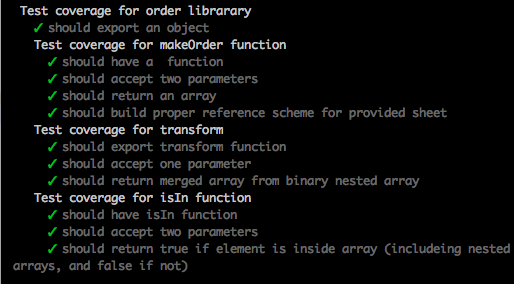
\includegraphics[width=\linewidth]{grafiken/testOrder.png}
	\caption{Test coverage for order.js}
	\label{fig:testOrder}
\end{figure}

\subsection{Correspondence to design principles}
\begin{itemize}
	\item Closing - nothing is likely to change;
	\item Code to an Interface - exports a single function;
	\item Do not repeat yourself - no code duplication;
	\item The Single-Responsibility Principle - nothing is likely to change;
	\item The Open/Closed Principle - no reason to change, no need for a new functionality;
	\item The Liskov Substitution Principle - no inheritance;
	\item The Dependency-Inversion Principle - does not have any lower level modules;
	\item The Interface Segregation Principle - does not have any lower level modules;
	\item Principles of Least Knowledge -  can be invoked only via direct import;
	\item Principle of Loose Coupling - exports a single function.
\end{itemize}

\section{Execution Schema}
In this step performed recursive replacement of respective elements in an \textit{execution order} array with elements from the \textit{scheme} object. The function (Listing: \ref{execScheme}) accepts two arguments: \textit{scheme} object and \textit{order} array. If an element is of an input array is an array it performs recursive call.

\lstinputlisting[
language=Javascript, numbers=left, stepnumber=5, firstnumber=1, breaklines=true, 
basicstyle=\footnotesize,
numberstyle=\tiny,
caption={Result of the scheme creation  for Test Sheet},
captionpos=b,
label=execScheme
]
{code/executionSchema.js.txt}
\subsection{Test Coverage}
Following test cases can show each step incrementally performed during the develop process.
\begin{figure}[H]
	\centering
	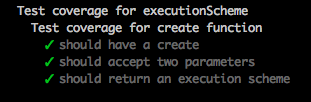
\includegraphics[width=\linewidth]{grafiken/testCreate.png}
	\caption{Test coverage for creation of execution scheme}
	\label{fig:testCreate}
\end{figure}

\subsection{Correspondence to design principles}
\begin{itemize}
	\item Closing - nothing is likely to change;
	\item Code to an Interface - exports a single function;
	\item Do not repeat yourself - no code duplication;
	\item The Single-Responsibility Principle - nothing is likely to change;
	\item The Open/Closed Principle - no reason to change, no need for a new functionality;
	\item The Liskov Substitution Principle - no inheritance;
	\item The Dependency-Inversion Principle - does not have any lower level modules;
	\item The Interface Segregation Principle - does not have any lower level modules;
	\item Principles of Least Knowledge -  can be invoked only via direct import;
	\item Principle of Loose Coupling - exports a single function.
\end{itemize}

\section{Template}
The translation to executable javascript file is made by apply the \textit{template} function. This function accepts three parameters \textit{sheet <Object>, scheme <Object>, fileName<String>}. \textit{Sheet} is a javascript object returned by reading the content of Test Sheet file. The \textit{scheme} is an execution order scheme. The \textit{fileName} is a path to the TestSheet file. This function creates a string content for javascript file based on provided parameters. The creation takes part in a four stages. 


The \textbf{first stage} is adding a description from the first element of the scheme object. It enclosed within the multiline comment symbols.


The \textbf{second stage} is adding require of reporting module for representation of execution of the tests result.


The \textbf{third stage} is adding declarations of the module scope variables. The variable names are taken from the coordinates of cells which store input and output parameters in a Test Sheet. The values of this variables are taken as from the cells with respective addresses.


The \textbf{fourth stage} is adding calls of the methods (Listing: \ref{template}). This stage is the most important part of this module. Since there are two types of execution orders adding function calls performed in a two steps. 


The \textit{\textbf{first step}} is adding calls for independent test steps. This is made be iterative call of \textit{makeCall} function with appending closing brackets to the end of the result string during each iteration. This function simply performs mapping between \textit{sheet} object (content of xlsx file), \textit{scheme} entry (test step) and string with content for executable javascript file (Listing: \ref{makeCall}).

\lstinputlisting[
language=Javascript, numbers=left, stepnumber=5, firstnumber=1, breaklines=true, 
basicstyle=\footnotesize,
numberstyle=\tiny,
caption={Function makeCall from template module},
captionpos=b,
label=makeCall
]
{code/makeCall.js.txt}

Note that functions in the generated code are not called directly but via \textit{call} method of the function's prototype. This method provides an opportunity to call the function from different context (environment). In current example the implementation of \textit{stack} module does not depend on the environment in which it was called. But in some cases the result of function's invocation can depend on the environment in which it was invoked. One of such cases can be creation of child process. The environment for such calls should be passed as a \textit{obcet under test}.


The \textit{\textbf{second step}} is adding calls for interdependent test steps. For every  element of \textit{nestedCalls} array it calls \textit{makeCall} function and if next element is an array this functions performs recursive call with appending of the closing brackets to the result of this call. In case if next element is not an array it appends closing brackets and performs next iteration.

%
%It is implemented as \textit{addCalls} function. This is recursive function which accepts four parameter: \textit{sheet, scheme, indentation, accumulator, fileName}. First two parameters are necessary to access the values represented in a Test Sheet. Next parameter is an indentation level which represents the deepness of a function call by adding representative amount of spaces for each line of generated code. Accumulator parameter is a string to which will be appended result of each recursive call of the function. The last parameter is necessary for report mechanism which allows to record result of the test execution to appropriate file. The report mechanism (e.g \textit{makeComparisonAndWriteResult}) will be described in details within  the next section. However it is important to mention here how it works as a 'black box'. It is binary function which accepts  six parameters. First parameter is an expected return value. Second is an actual returned value received by the callback function, third is a deepness of comparison will be performed for this their values. The function returns \textbf{true} in case of match and after redefinition of the variable takes place. This mechanism allows usage of references within the Test Sheet for asynchronous functions.
%\lstinputlisting[
%language=Javascript, numbers=left, stepnumber=5, firstnumber=1, breaklines=true, 
%basicstyle=\footnotesize,
%numberstyle=\tiny,
%caption={Function addCalls from template module},
%captionpos=b,
%label=template
%]
%{code/lib/template/template.js.txt}




\subsection{Test Coverage}
Following test cases can show each step incrementally performed during the develop process.

%\lstinputlisting[
%language=Javascript, numbers=left, stepnumber=5, firstnumber=1, breaklines=true, 
%basicstyle=\footnotesize,
%numberstyle=\tiny,
%caption={Test coverage for creation of the Test Sheet template},
%captionpos=b,
%label=writeIn
%]
%{code/test/template.js.txt}

The result of test execution:
\begin{figure}[H]
	\centering
	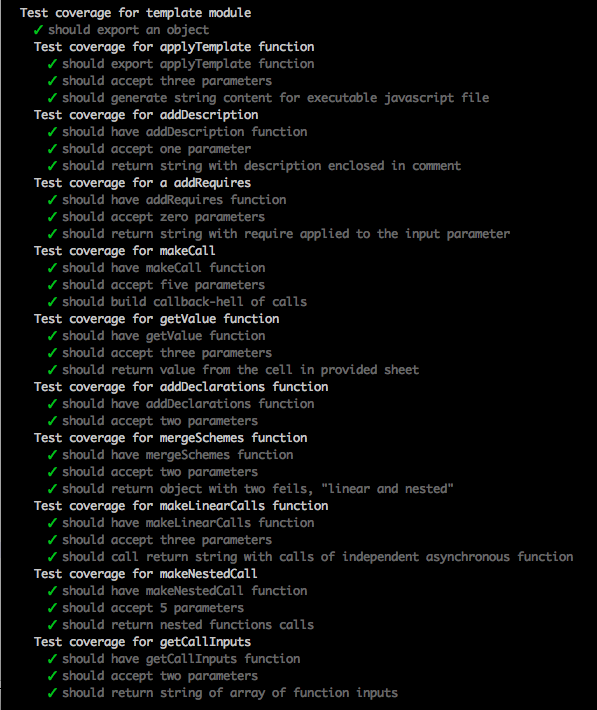
\includegraphics[width=\linewidth]{grafiken/testTemplate.png}
	\caption{Test coverage for template.js}
	\label{fig:testTemplate}
\end{figure}

\subsection{Correspondence to design principles}
\begin{itemize}
	\item Closing - content generation is enclosed within three independent functions;
	\item Code to an Interface - exports a single function;
	\item Do not repeat yourself - no code duplication;
	\item The Single-Responsibility Principle - can be changed only due to the requirements for generated code;
	\item The Open/Closed Principle - no need to be changed;
	\item The Liskov Substitution Principle - no inheritance;
	\item The Dependency-Inversion Principle - does not have any lower level dependencies;
	\item The Interface Segregation Principle - does not have any lower level dependencies;
	\item Principles of Least Knowledge - can be invoked only via direct import;
	\item Principle of Loose Coupling - exports a single function.
\end{itemize}

\section{Write Stream}

This part of the system implements on function and exports it wrapped in to object stream. It receives an object from the up stream with following structure (Lisitng: \ref{writeIn}). It tries to read meta data of the file with same name as Test Sheet file but with the .js extension, it possible only if the file exists. In other case, the exception will be thrown and caught by catch block which implements creation of the file with content received from the up stream, and notification of user about successfully created file via standard system output or an error if the file failed to create. If file already exists the function will be able to read its meta data. After it, this meta data will be compared with meta data of the Test Sheet file received from the upstream. In case if modification date of the Test Sheet file is bigger then modification data of javascript file system will overwrite the javascript file with content received from the upstream. In other case case (Tests sheet file was not updated after creation of representative javascript file) the system will switch to the next object received from the up stream. The result javascript file generated from the provided Test Sheet looks as following (Listing: \ref{demo})

\lstinputlisting[
language=Javascript, numbers=left, stepnumber=5, firstnumber=1, breaklines=true, 
basicstyle=\footnotesize,
numberstyle=\tiny,
caption={Generated javascript file},
captionpos=b,
label=demo
]
{code/demo/demo.js.txt}

%\lstinputlisting[
%language=Javascript, numbers=left, stepnumber=5, firstnumber=1, breaklines=true, 
%basicstyle=\footnotesize,
%numberstyle=\tiny,
%caption={write\_stream.js},
%captionpos=b,
%label=demo
%]
%{code/lib/stream/writeStream.js.txt}

\subsection{Test Coverage}
Following test cases can show each step incrementally performed during the develop process. All calls to systems I/O (e. g. read file meta data, read file) are implemented using stubs.
%\lstinputlisting[
%language=Javascript, numbers=left, stepnumber=5, firstnumber=1, breaklines=true, 
%basicstyle=\footnotesize,
%numberstyle=\tiny,
%caption={Test coverage for write\_stream.js},
%captionpos=b,
%label=writeTest
%]
%{code/test/writeStream.js.txt}


The result of tests execution  for this module is following (Fig.: \ref{fig:testWrite}): 
\begin{figure}[H]
	\centering
	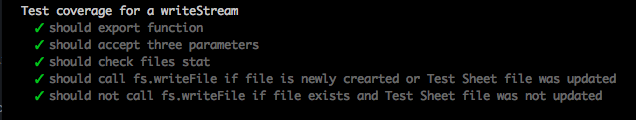
\includegraphics[width=\linewidth]{grafiken/testWriteStream.png}
	\caption{Test coverage for write\_stream.js}
	\label{fig:testWrite}
\end{figure}

\subsection{Correspondence to design principles}
\begin{itemize}
	\item Closing - module exports single stream object with wrapped function.
	\item Code to an Interface - calls are done to the public functions of required objects. 
	\item Do not repeat yourself - small code duplication in callbacks for file writing, avoiding which will add more complexity;
	\item The Single-Responsibility Principle - can be changed only due to the change of output type (e. g. another output file extension)
	\item The Open/Closed Principle - performs writing to the file only;
	\item The Liskov Substitution Principle - no inheritance;
	\item The Dependency-Inversion Principle - 
	\begin{itemize}
		\item Higher level module \textit{index.js} does not depend on implementation current library
		\item Current library depends on the input type provided by the \textit{index.js}
	\end{itemize}
	\item The Interface Segregation Principle - no calls of unnecessary methods;
	\item Principles of Least Knowledge - communication done only with js files;
	\item Principle of Loose Coupling - communication is done via standard file system and standard stream interfaces.
\end{itemize}

\section{Reporting mechanism}
The reporting mechanism made as a standalone npm package which must me installed globally for being available at any place of the system where it is called by generated javascript files described in a previous section. 
The folder/file structure of the application looks as following:
\begin{itemize}
	\item index.js
	\item package.json
	\item ReadMe.md
	\item lib/
	\begin{itemize}
		\item compare\_and\_write.js
	\end{itemize}
	\item test/
	\begin{itemize}
		\item compare\_and\_write.js
	\end{itemize}
	\item node\_modules/
\end{itemize}

\subsection{Implementation}
\lstinputlisting[
language=Javascript, numbers=left, stepnumber=5, firstnumber=1, breaklines=true, 
basicstyle=\footnotesize,
numberstyle=\tiny,
caption={Report mechanism's main function},
captionpos=b,
label=report
]
{code/report.js.txt}

\begin{figure}[H]
	\centering
	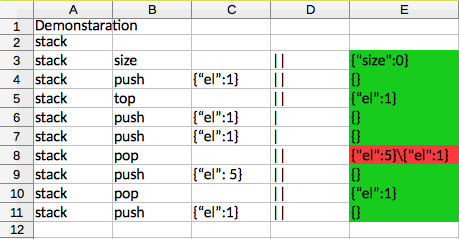
\includegraphics[width=\linewidth]{grafiken/testSheetResult.png}
	\caption{Result Test Sheet for stack.js}
	\label{fig:resultTestSheet}
\end{figure}


\subsection{Test coverage}
Following test cases can show each step incrementally performed during the develop process. All calls to systems I/O (e. g. read file meta data, read file) are implemented using stubs.
The result of tests execution  for this module is following (Fig.: \ref{fig:testReport}): 
\begin{figure}[H]
	\centering
	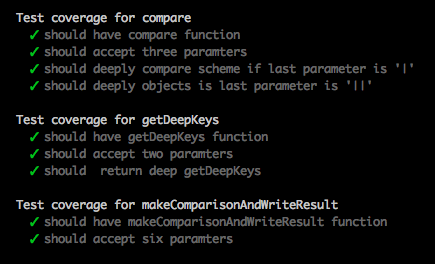
\includegraphics[width=\linewidth]{grafiken/testReport.png}
	\caption{Test coverage for report mechanism}
	\label{fig:testReport}
\end{figure}

\subsection{Correspondence to design principles}
\begin{itemize}
	\item Closing - comparison and reporting are done in a different independent functions
	\item Code to an Interface - exports a single function;
	\item Do not repeat yourself - no code duplication;
	\item The Single-Responsibility Principle - can be changed only due to the reporting media;
	\item The Open/Closed Principle - new functionality can be added as another exported function;
	\item The Liskov Substitution Principle - no inheritance (required as an npm package);
	\item The Dependency-Inversion Principle - requires standard \textit{assert}, \textit{files system} modules and \textit{xlsx} module;
	\item The Interface Segregation Principle - does not have any lower level modules;
	\item Principles of Least Knowledge -  can be invoked only via direct import;
	\item Principle of Loose Coupling - exports a single function.
\end{itemize}